

\chapter{Einleitung}
\lohead{ReShuffled Projektplanung}

\section{Das Projektteam}
\label{sec:Einleitung}

\begin{figure}[H]
    \vspace{-30pt}
    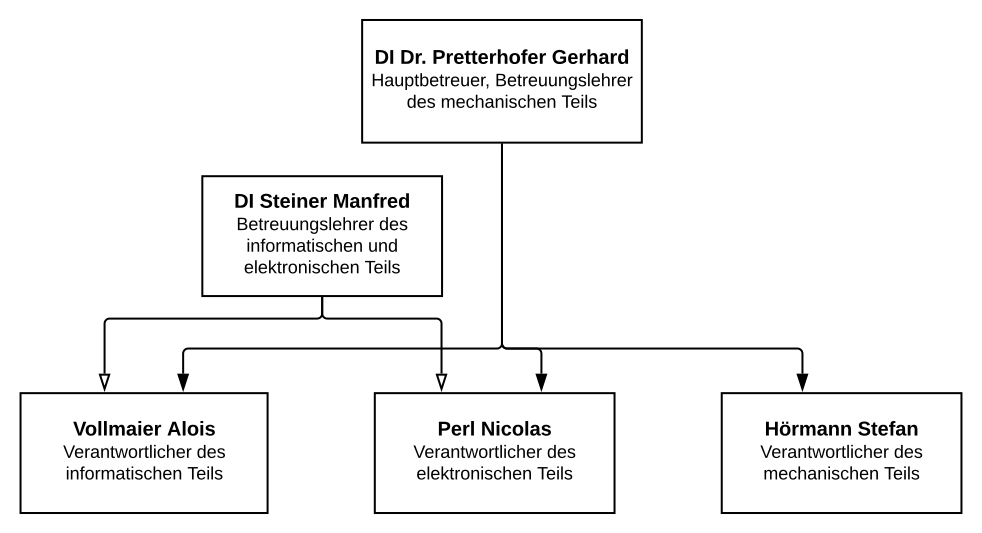
\includegraphics[width=0.80\textwidth]{fig/Hierachie_Reshuffled.pdf}
    \caption{Betreuerübersicht}
    \label{Bild über ganze Seitenbreite}
\end{figure}


\section{Konzept}
Wir setzten uns als Ziel eine Maschine zu entwickeln, welche das Mischen, sowie das Ausgeben von Spielkarten übernimmt.
Die Idee ist es, diese Verfahren möglichst platzsparend, zeiteffizient und detailliert durchdacht und optimiert zu realisieren.\\

\begin{wrapfigure}{r}{0.34\textwidth}
    \vspace{-40pt}
    \begin{center}
        \includegraphics[width=0.35\textwidth]{fig/Reshuffled_Version_3_prinzip}
    \end{center}
    \caption{Kartenentnahme}
    \label{Kartenentnahme}
    \vspace{-15pt}
\end{wrapfigure}

Grundsätzlich basiert das Mischprinzip auf einer Art "Fächersystem".
Eingelegte Karten gelangen mithilfe eines ausgeklügelten Systems, welches aus einem Hubmagneten mit integriertem Saugnapf besteht, aus dem Einlegefach.
Erfolgt die Kartenentnahme, rutscht die Karte in ein zufälliges Fach des Lagerrads. Anschließend wird dieses Lagerrad in Drehbewegung versetzt um die gelagerten Karten auszugeben.

Der Benutzer steuert diese Maschiene auf einer GUI welche auf einem 7" LCD Display angezeigt wird. Systemintern steuert ein 8Bit Mikrocontroller der AVR-Familie den Ablauf.

%============================================
\chapter{Mechanik}
\lohead{Stefan Hörmann}
\label{sec:Mechanik}
\section{Beschreibung}

Der mechanische Teil begann mit dem Variantenvergleich, dabei wurden verschiedene Varianten der Maschine basierent auf deren Kosten, deren Schnelligkeit und deren Realisierbarkeit verglichen.
Auch muss daruf geachtet werden, dass die benötigten Bauteile weitestgehend in der Schule oder Privat gefertigt werden können.\\

\begin{wrapfigure}{r}{0.5\textwidth}
    \vspace{-50pt}
    \begin{center}
        \includegraphics[width=0.5\textwidth]{fig/Reshuffled_Version_3_0_prinzip}
    \end{center}
    \caption{Variantenvergleich Version 3}
    \label{Variantenvergleich}
    \vspace{-15pt}
\end{wrapfigure}

Danach wurde der Motor ausgewählt, dies erfolgte über diverse Berechnungen die die einwirkenden Kräfte auf das Lagerrad sowie dei benötigten Beschleunigungskräfte berücksichtigten.
Wurde dies erledigt, wird der Hubmagnet ausgewählt. Dabei wurde auf die Bauform, auf die Art des Aufbaus und den Preis geachtet.
\\\\
Die CAD-Zeichnungen des Lagerrads sollten vor den Ferien fertiggestellt werden und für die Werstatt freigegeben werden, sodass diese noch vor den Ferien für Testdurchläufe des Motors zur Verfügung stehen.
Auch die 3D-Druck Teile sollten vor den Ferien gedruckt sein.
\\\\
Der größte Teil der Arbeit besteht in der Konstruktion der gestamten Maschine, da die Teile hauptsächlich gedruckt werden, muss darauf geachtet werden, dass alle Teile so konstruiert werden das dies ohne Probleme funktioniert.
Für die CAD-Konstrucktion wird das bereits in der Schule gelernte Programm Inventor benutzt, auch alle im nachhinein benötigten Belastungsanalysen sowie Simulationen werden mit diesem Programm erledigt.


%============================================
\chapter{Elektronik}
\lohead{Nicolas Perl}
\label{sec:Elektronik}
\section{Beschreibung}

TODO



%============================================
\chapter{Informatik}
\lohead{Alois Vollmaier}
\label{sec:Informatik}
\section{Beschreibung}

Den Informatischen Teil der Arbeit kann man grundsätzlich in 2 Bereiche aufteilen. Einerseits soll eine einfache grafische Benutzeroberfläche gestaltet werden, auf welcher man den Mischvorgang steuern sowie grundlegende Einstellungen des Spieles vornehmen kann.
Aus programmtechnischen Gründen wird hierfür die Programmiersprache Java und das GUI-Toolkit Swing verwendet. \\
Die Hardwarekomponenten setzten sich aus einem Raspberry Pi 3B+ und einem 7" LCD Touchscreen der Firma Elecrow zusammen. \\

Andererseits besteht dieser Teilbereich der Arbeit auch aus der hardwarenahen Programmierung der Hauptplatine. Mithilfe der Programmiersprache C sollte der verbaute 8Bit Mikrocontroller der AVR-Familie namens ATmega 324P programmiert werden.
Dieser steuert den gesamten Ablauf der Maschiene. \\

Der Datenaustausch zwischen Hauptplatine und Raspberry PI erfolgt über die serielle Schnittstelle namens UART.
Im Hintergrund wird gleichzeitig eine Json Logdatei
%============================================
\chapter{Projektplanung}
\lohead{ReShuffled Projektplanung}
\label{sec:Projektplanung}
\section{Meilensteine}
\begin{table}[h!]
    \begin{tabular}{ll}
        \hline
        \rowcolor[HTML]{C0C0C0}
        \multicolumn{2}{c}{\cellcolor[HTML]{C0C0C0}\textbf{Meilensteine}}                      \\ \hline
        \rowcolor[HTML]{EFEFEF}
        \multicolumn{1}{l|}{\cellcolor[HTML]{EFEFEF}Datum} & Beschreibung                      \\ \hline
        \multicolumn{1}{l|}{15. Mai 2019}                   & Vollenden des Variantenvergleichs \\ \hline
        \multicolumn{1}{l|}{01. Aug.2019}                    & Fertigstellung der CAD Zeichnung  \\ \hline
        \multicolumn{1}{l|}{15. Sep. 2019}                   & Fertigstellung der Hardware       \\ \hline
        \multicolumn{1}{l|}{31. Okt. 2019}                   & Abschließen des Testaufbaus       \\ \hline
        \multicolumn{1}{l|}{01. Dez. 2019}                    & Fertigstellung der Software       \\ \hline
    \end{tabular}
\end{table}

\section{Aufgabenplanung bis September}

Ziele des Herrn Hörmann:
\begin{itemize}
    \item Standartmäßig ist ein schwarzer Punkt davor.
    \item Die Länge ist nicht von Bedeutung, Zeilen werden automatisch umgebrochen.
\end{itemize}

\noindent\hrulefill

Ziele des Herrn Pearl:
\begin{itemize}
    \item Standartmäßig ist ein schwarzer Punkt davor.
    \item Die Länge ist nicht von Bedeutung, Zeilen werden automatisch umgebrochen.
\end{itemize}

\noindent\hrulefill

Ziele des Herrn Vollmaier:
\begin{itemize}
    \item Standartmäßig ist ein schwarzer Punkt davor.
    \item Die Länge ist nicht von Bedeutung, Zeilen werden automatisch umgebrochen.
\end{itemize}

%============================================
\chapter{Anhang}




